\documentclass[12pt]{article}
\usepackage{amsmath} % flere matematikkommandoer
\usepackage{amssymb}
\usepackage[utf8]{inputenc} % æøå
\usepackage[T1]{fontenc} % mere æøå
\usepackage[danish]{babel} % orddeling
\usepackage{verbatim} % så man kan skrive ren tekst
\usepackage[all]{xy} % den sidste (avancerede) formel i dokumentet
\usepackage{graphicx}
\usepackage{algorithm}
\usepackage[noend]{algpseudocode}
\usepackage{listings}

\lstset{
  basicstyle=\ttfamily\scriptsize,
  breaklines=true,
  tabsize=2
}

\def\BState{\State\hskip-\ALG@thistlm}

\title{AlgDat genaflevering 2\\af task 2, 3 og 5}
\author{Nicklas Warming Jacobsen - qmr656\\Simon Warg - bcs315\\Robert Rasmussen - dfs207\\Christian Enevoldsen - mbr852}
\date{D. 23. Maj 2014}
\begin{document}
\maketitle
\newpage
\section*{Task 1}
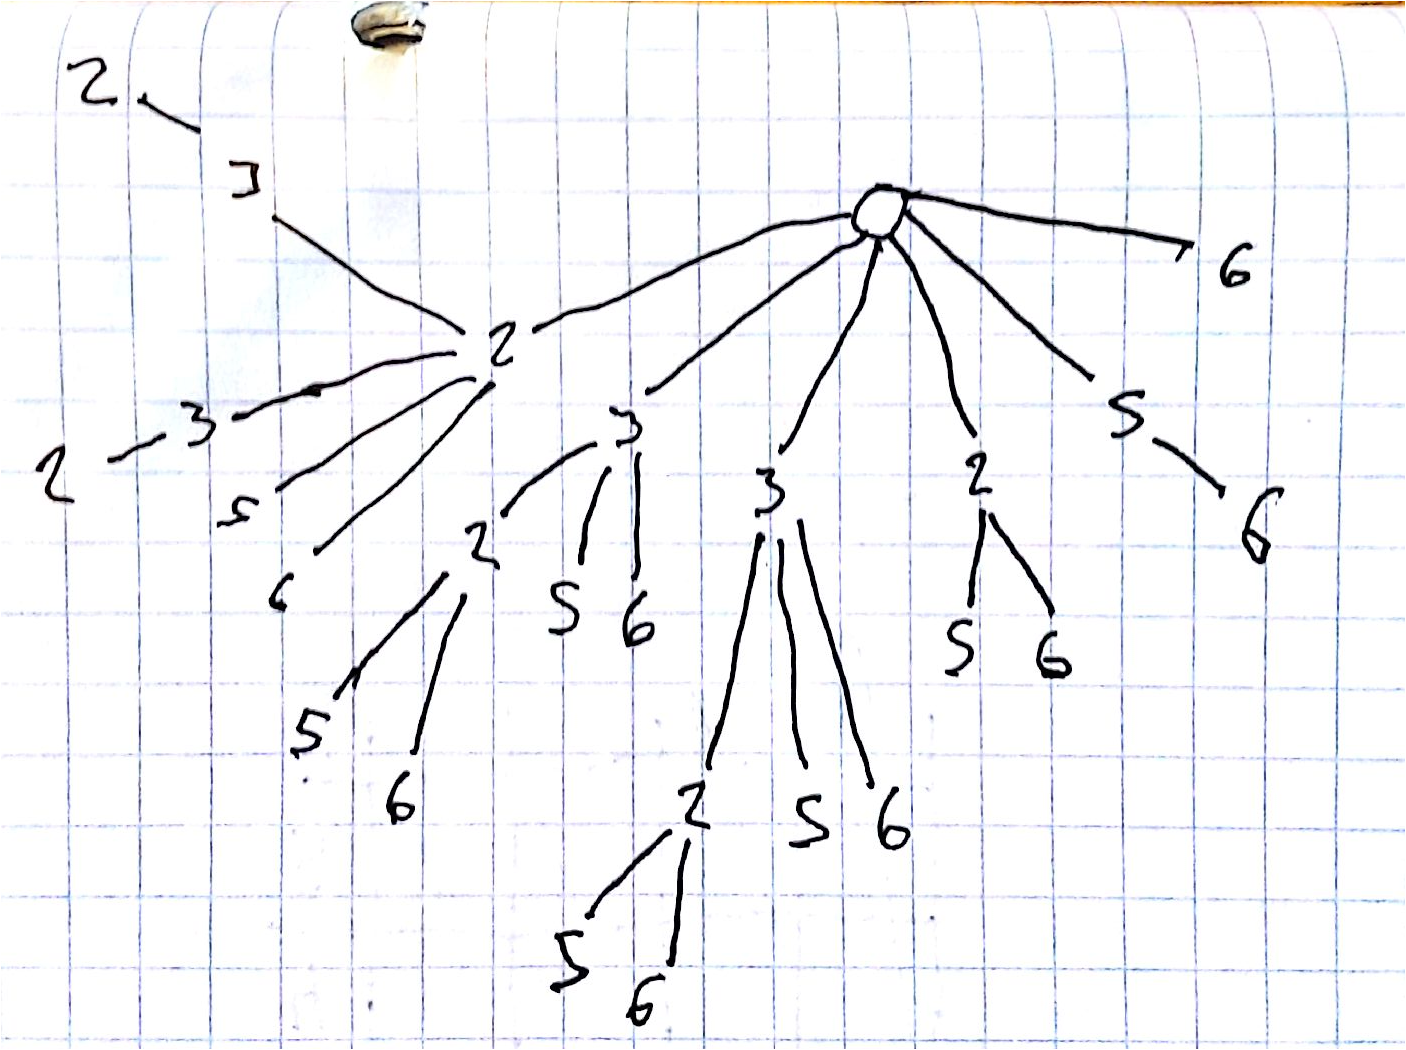
\includegraphics[width=13cm]{tree.png}\\
Overstående graf er en graf over alle zigzag sekvenserne for $A=\{2,3,3,2,5,6\}$. Man kan se at vi i flere udgreninger finder en optimal sub-sekvens. Derudover finder man sub-problemer som bliver løst flere gange (de overlapper hinanden.), f. eks. er subproblemerne for $3$ identiske og sekvensen $\{2,3,2\}$ optræder flere gange.
\newpage
\section*{Task 2}
\lstinputlisting{lzg.py}
\section*{Task 3 - Loop invariance}
\subsection*{Initianlization}
Ved $n=0$ er den trivielle løsning 0, som retuneres. Ved $n > 0$ sættes c (vores delresultat) til $c = 1$, dette er sandt da det er den længste zigzag sekvens for dellisten af $A$, med det første element.
Vores invariance holder derfor inden løkken.
\subsection*{Maintenance}
Vi ser at hvis det er det første loop og det næste element i listen $a$ ikke er det samme som det nuværende, eller der sker et zigzag så tæller vi op og differencen bliver gemt til næste iteration.
Ellers ser vi at vi ikke tæller op, men derimod kun gemme differencen til næste iteration hvis den er absolut større.
\subsection*{Termination}
For hver iteration bliver $i$ én større, loopet må derfor slutte når $i = n$. Og da vi har gjort c én større hver gang vi har ramt et zigzag, må c = lzg(a)
\section*{Task 4}
\subsection*{Hukommelse}
Da algoritmen ikke laver et nyt array, og tager i mod et af array af længde $n$, så kræver algoritmen $O(n+k)$ hukommelse hvor k er en konstant faktor, dvs. algoritmen kræver $O(n)$ hukommelse.
\subsection*{Tid}
Da der kun er ét loop der køre $n$ gange, så køre algoritmen i $O(n)$ tid.
\subsection*{Task 5}
\lstinputlisting{showLzg.py}
\section*{Exam subject outline - Nicklas Jacobsen qmr656}
De fire generale step i konstruktionen af en dynamisk programerings algoritme er:
\begin{enumerate}
  \item{Karakterisere strukturen i en optimal løsning}
  \item{Rekursivt finde de optimale løsninger til delproblemerne}
  \item{Beregne den optimale værdi for det overordnede problem}
  \item{Konstruerer en optimal løsning til fra den beregnede information}
\end{enumerate}
De tre krav til dynamistisk programerings algoritmer:
\begin{enumerate}
  \item{For at man kan bruge dynamisk programering, skal de optimale løsninger til sub-problemerne være en delmængde af den optimale løsning til det oprindelige problem.}
  \item{To sub-problemer til det samme problem skal være uafhænige af hinanden.}
  \item{Sub-problemerne skal overlappe hinanden, dvs. mængden af forskellige sub-problemer skal være relativ lille (modsat f. eks. divide and conquer hvor man generer nye sub-problemer ved hvert step.)}
\end{enumerate}
\subsection*{LCS eksempel}
LCS er den længste fælles del-sekvens af to stringe.
Hvis vi har to stringe $X = \{x_1, x_2...,x_m\}$ og $Y=\{y_1, y_2...,y_n\}$ og deres LCS $Z=\{z_1, z_2...z_k\}$, så gælder det at:
\subsubsection*{Optimal sub-struktur}
\begin{enumerate}
  \item{Hvis $x_m=y_n$, så $z_k=x_m=y_n$ og $Z_k-1$ er en LCS af $X_{m-1}$ og $Y_{n-1}$}
  \item{Hvis $x_m \neq y_n$, så $z_k \neq x_m$ som indikerer at $Z$ er en LCS af $X_{m-1}$ og $Y$}
  \item{Hvis $x_m \neq y_n$, så $z_k \neq y_n$ som indikerer at $Z$ er en LCS af $Y_{n-1}$ og $X$}
\end{enumerate}
\textbf{\textit{Bevis 1}}
\textit{Første del:}\\
Hvis $x_m=y_n$ og $x_m\neq z_k$ så kunne vi tilføje $x_m=y_n$ til $Z$ og få en LCS af $X$ og $Y$ på længden $k+1$, hvilket ville være i modstrid med at $Z$ er en LCS af $X$ og $Y$. Det må derfor være at hvis $x_m=y_n$ så $z_k=x_m=y_n$.\\
\textit{Anden del:}
Vi ønsker at bevise at hvis $x_m=y_n$ så er $Z_{k-1}$ en LCS af $X_{m-1}$ og $Y_{n-1}$. Med formål for modstrid antager vi, at der eksisterer en fælles sekvens $W$ for $X_{m-1}$ og $Y_{n-1}$ som har en længde større end $k-1$. Hvis vi tilføjer $x_m=y_n$ til $W$ resulterer det i en fælles sekvens for $X$ og $Y$, med en længde større end $k$, hvilket er i modstrid med at $Z$ er en LCS.
\\\\\textbf{\textit{Bevis 2 og vice versa for 3}}
Hvis $x_m \neq z_k$ så er $Z$ en LCS af $X_{m-1}$ og $Y$, for hvis der eksisterer en fælles sekvens $W$ for $X_{m-1}$ og $Y$ med længde større end k, så vil $W$ også være en LCS af $X$ og $Y$, hvilket ville være i modstrid med at $Z$ er en LCS af $X$ og $Y$.\\\\
Overstående viser at LCS problemet har en optimal-substruktur.
\subsubsection*{Overlappende sub-problemer}
Ved at kigge på de tre punkter under ``Optimal sub-struktur'', kan man se at for at finde LCS af $X$ og $Y$ skal vi håndtere en ud af to situationer:\\
1: Hvis $x_m=y_n$ så skal vi finde LCS for $X_{m-1}$ og $Y_{n-1}$, og ved at tilføje $x_m=y_n$ til denne får vi LCS af $X$ og $Y$.\\
2: I tilfældet af at $x_m\neq y_n$, skal vi løse to problemer. Vi skal finde LCS af $X_{m-1}$ og $Y$, og vi skal finde LCS af $X$ og $Y_{n-1}$, og retunerer den LCS der er længst.\\
Det tydeligt at se at vi kommer til at løse de samme sub-problemer flere gange.

\subsubsection*{Resultat}
\begin{tabular}{ c|c|c|c|c|c}
  &j&0&1&2&3\\ \hline
  i&&&\textbf{A}&\textbf{D}&\textbf{C}\\ \hline
  0&&0&0&0&0\\ \hline
  1&\textbf{A}&0&$\nwarrow$ 1&$\leftarrow$1&$\leftarrow$1\\ \hline
  2&C&0&$\uparrow$1&$\leftarrow$1&$\nwarrow$2\\ \hline
  3&\textbf{D}&0&$\uparrow$1&$\nwarrow$2&$\leftarrow$2\\ \hline
  4&A&0&$\nwarrow$1&$\uparrow$2&$\leftarrow$2\\ \hline
  5&\textbf{C}&0&$\uparrow$1&$\uparrow$2&$\nwarrow$3\\
\end{tabular}\\
Tabellen ovenfor viser resultatet af en dynamisk programmerings algortime til at beregne LCS af to stringe i og j.
For at aflæse tabellen, starter man nede i nederste højre hjørne og følger pilene. Hver gang man møder $\nwarrow$ tilføjer man det pågældende bogstav til sin LCS.
\newpage
\section*{Exam subject outline - Robert Rasmussen - dfs207}
\section{Points}
\begin{itemize}
\item Optimal substructure
\item Overlapping subproblems
\item Memoization
\item Top-down
\item Bottom-up 
\end{itemize}

\section{Problem Instance}
How the bottom-up-cut-rod algorithm works.
\end{document}
